%%================================================
%% Filename: chap05.tex
%% Encoding: UTF-8
%% Author: 苏峻锋
%%================================================
\chapter{预测模型与传统负载均衡的结合}
回顾第二章的讨论,我们已经详细分析了传统负载均衡策略的工作原理,虽然这些传统策略在多种场景下都能提供稳定的性能,但在面对动态变化和未预见负载的情况时,仍然显得力不从心。本章旨在探讨一种新的解决方案,即预测模型与传统负载均衡的结合,以期望克服现有方法的不足。我们将首先介绍结合方案的设计理念与实施策略,随后通过实验验证其有效性,并对模型的表现进行深入分析。

\section{传统负载均衡算法的选取}
在第二章的讨论中,发现了加权轮询算法原理简单,而且配置比较简便,权重可以很好的反映出集群内服务器节点的性能和负载情况,是一种非常经典的负载均衡算法。本文选择以加权轮询算法为基础,分析其原理并进行改进,实现一种检测服务器节点负载状况,并以此为根据动态地调整各个节点权重以合理分配请求任务目的的算法。

相比于默认的轮询算法,加权轮询算法则考虑了不同性能特点的服务器节点,性能好的服务器则设置较大的权值,
性能不好的服务器则设置较小的权值。
当任务入队列时负载均衡器则可以按照设置好的权值比例合理的悬着服务器执行任务请求。

通过对 Nginx 源码的研究,在 ngx\_http\_upstream\_round\_round\_robin.c 这个文件下 ngx\_http\_upstream\_get\_round\_robin\_peer
函数是对加权轮询算法的实现。在具体分配任务的环节,为了记录上游集群节点服务器的权值公设有四个变量,
依次是 weight、effective\_weight、total 和 current\_weight。

\noindent\begin{longtblr}
  [caption = {加权轮询算法变量及描述}]
  {hlines, colspec = {|X[1, c]|X[2, c]|}}
  变量 & 描述 \\
  weight & 初始权值,固定不变 \\
  effective\_weight & 发生错误,权值减小 \\
  total & 集群服务器权值总和 \\
  current\_weight & 实时权值,初始为零 \\
\end{longtblr}

在一次任务中,负载均衡器勉励上游服务器节点的 current\_weight 加上起对应的有效权值 effective\_weight,
负载均衡器将会选择 current\_weight 最大的服务器节点为本轮最佳服务器。当该服务器正在进行任务时,负载均衡器会
降低其 current\_weight。Nginx 定义了两个事件状态,NGX\_OK 表示成功选择最佳服务器,NGX\_BUSY 表示服务器选择失败
或者通信发生错误。加权轮询算法详细流程如下图\ref{weight_round}所示。

\begin{figure}[htb]
  \centering
  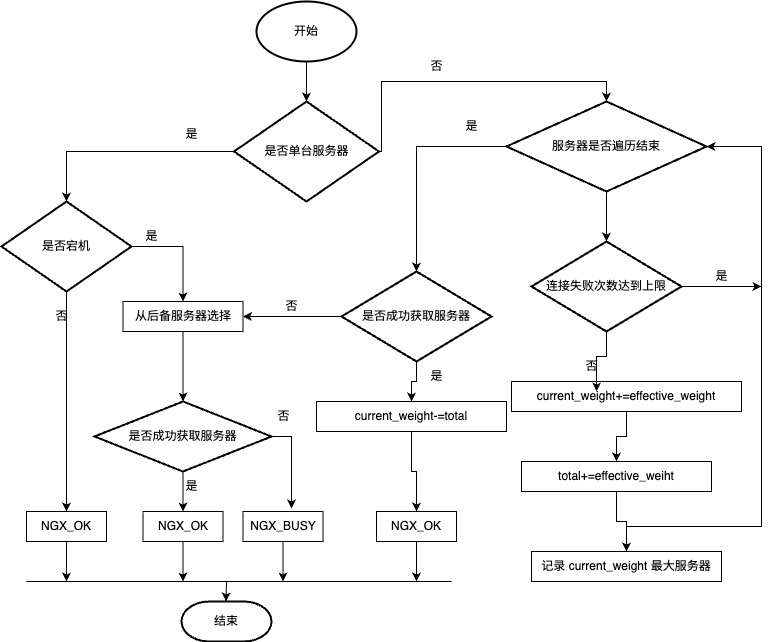
\includegraphics[width=\textwidth]{figures/round-flowchart.jpg}
  \caption{Nginx 加权轮询算法流程图}
  \label{weight_round}
\end{figure}

加权轮询算法,虽然考虑了上游服务器节点的不同性能差异,执行效率较高,节点选择频次相对平滑,
配置简单,但是在具体任务过程中,有些任务比较繁忙,有些任务比较轻松,这种静态的权重调节无法根据真实负载
情况进行动态调整。为了解决这个问题,诞生了动态权值的加权轮询算法,基于手机各个后台服务器节点工作时的 CPU
利用率、内存利用率、网络性能和磁盘IO等性能情况,动态的调整后端服务器节点权重\cite{谭畅2021云中心基于}。该算法在高并发
的场景下,响应时间和实际并发方面表现更好。

常规的加权轮询算法在某些特殊的权重下,加权轮询调度会生成不均匀的实例序列,这种不平滑的负载可能会使某些实例出现瞬时高负载的现象,导致系统存在宕机的风险。
为了解决这个调度缺陷,就提出了平滑加权轮询调度算法。如图\ref{pinghualunxun}所示为 Nginx 中该算法的流程图。

\begin{figure}[htbp]
  \centering
  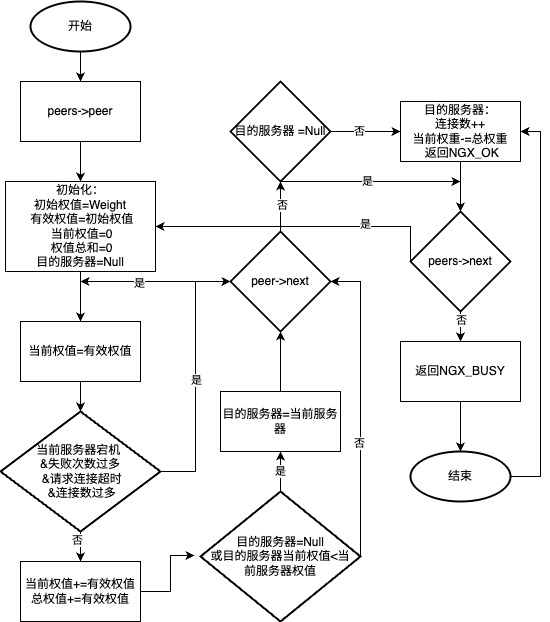
\includegraphics[width=.8\textwidth]{figures/smooth_weight.jpg}
  \caption{Nginx 内置平滑轮询算法流程图}
  \label{pinghualunxun}
\end{figure}

为了证明平滑性,只要证明不要一直都是连续选择那一个节点即可。假设总权重为 S,假如某个节点 i 连续选择了 t($t < x_i$) 次,只要存在下一次选择的不是节点 i,即可证明是平滑的。

假设 $t = x_i - 1$,此时第 i 个结点的当前权重为 $w_i = t \* x_i - t \* S = (x_i - 1) \* x_i - (x_i - 1) \* S$。即证明下一轮的第 1 步执行完的值 $w_i + x_i$ 不是最大。
\begin{equation}
  w_i + x_i => (x_i - 1) \* x_i - (x_i - 1) \* S + x_i =>x_i^2 - x_i \* S + S => (x_i - 1) \* (x_i - S) + x_i
\end{equation}

因为 $x_i$ 恒小于 S,所以 $x_i - S <= -1$。所以上面:$(x_i - 1) \* (x_i - S) + x_i <= (x_i - 1) \* -1 + x_i = -x_i + 1 + x_i = 1$。所以第 t 轮后,再执行完第 1 步的值 $w_i + x_i <= 1$。如果这 t 轮刚好是最开始的 t 轮,则必定存在另一个结点 j 的值为 $x_j \* t$,所以有 $w_i + x_i <= 1 < 1 \* t < x_j \* t$。所以下一轮肯定不会选中 i。

平滑加权轮询算法改善了加权轮询算法调度的缺陷,即调度序列分散的不均匀,避免了实例负载突然加重的可能,但是仍然不能动态感知每个实例的负载。若由于实例权重配置不合理,或者一些其他原因加重系统负载的情况,平滑加权轮询都无法实现每个实例的负载均衡,这时就需要有状态的调度算法来完成。由此本文在该算法基础上进行了相关调整,首先采集后台各个节点指标数据,包括 CPU、内存、网络带宽以及磁盘I/O指标数据,并对采集到的数据惊醒相关处理,通过这些数据来确定不同节点的初始权重,反应不同节点的初始性能差异。并持续周期性的收集综合负载指标,使用训练好的模型预测剩余性能,并根据该性能调整节点权重。同时为了防止初期无法得到有效的服务器负载均衡后的有效数据,将会使用默认的平滑加权算法来得到初期数据,经过一定周期,将收集到的负载均衡数据整理并使用预测模型进行预测,并根据预测的数据进行初始权重的调整和优化。

\section{改进的负载均衡算法的提出}
本次改进后的算法主要分为四个模块:服务器负载信息收集模块,服务器信息处理模块,Nginx 动态加权轮询模块,周期预测模块。四个模块协同完成改进的动态加权轮询算法的功能。其中负载均衡负载信息收集模块一直运转在各个集群节点中,负载周期性的获取各个节点的负载数据并存入 Memcached 中,包含访问次数,CPU、内存、网络带宽以及磁盘IO等利用率。
服务器信息处理模块在Nginx负载均衡的服务器上,从 Memcached 中获取各个节点的负载数据,并根据获取到的负载数据得到各个节点的综合负载情况,
根据设定的阈值 M 和 N 相比较,判断是否负载正常。如果节点负载过高或者过低,负载均衡服务器会调整该节点的权重,并将调整后的权重保存在 Memcached 服务中。另外,在周期预测性模块中,会周期性的以网站访问量以及综合负载指标来进行预测,调整阈值 M 和 N。
Nginx 动态加权轮询模块从 Memcached 中获取各个节点的最新权重信息,按照改进后的算法选取某一节点完成任务请求。系统总体结构如下图\ref{total_structure_flow}所示。

\begin{figure}[htbp]
  \centering
  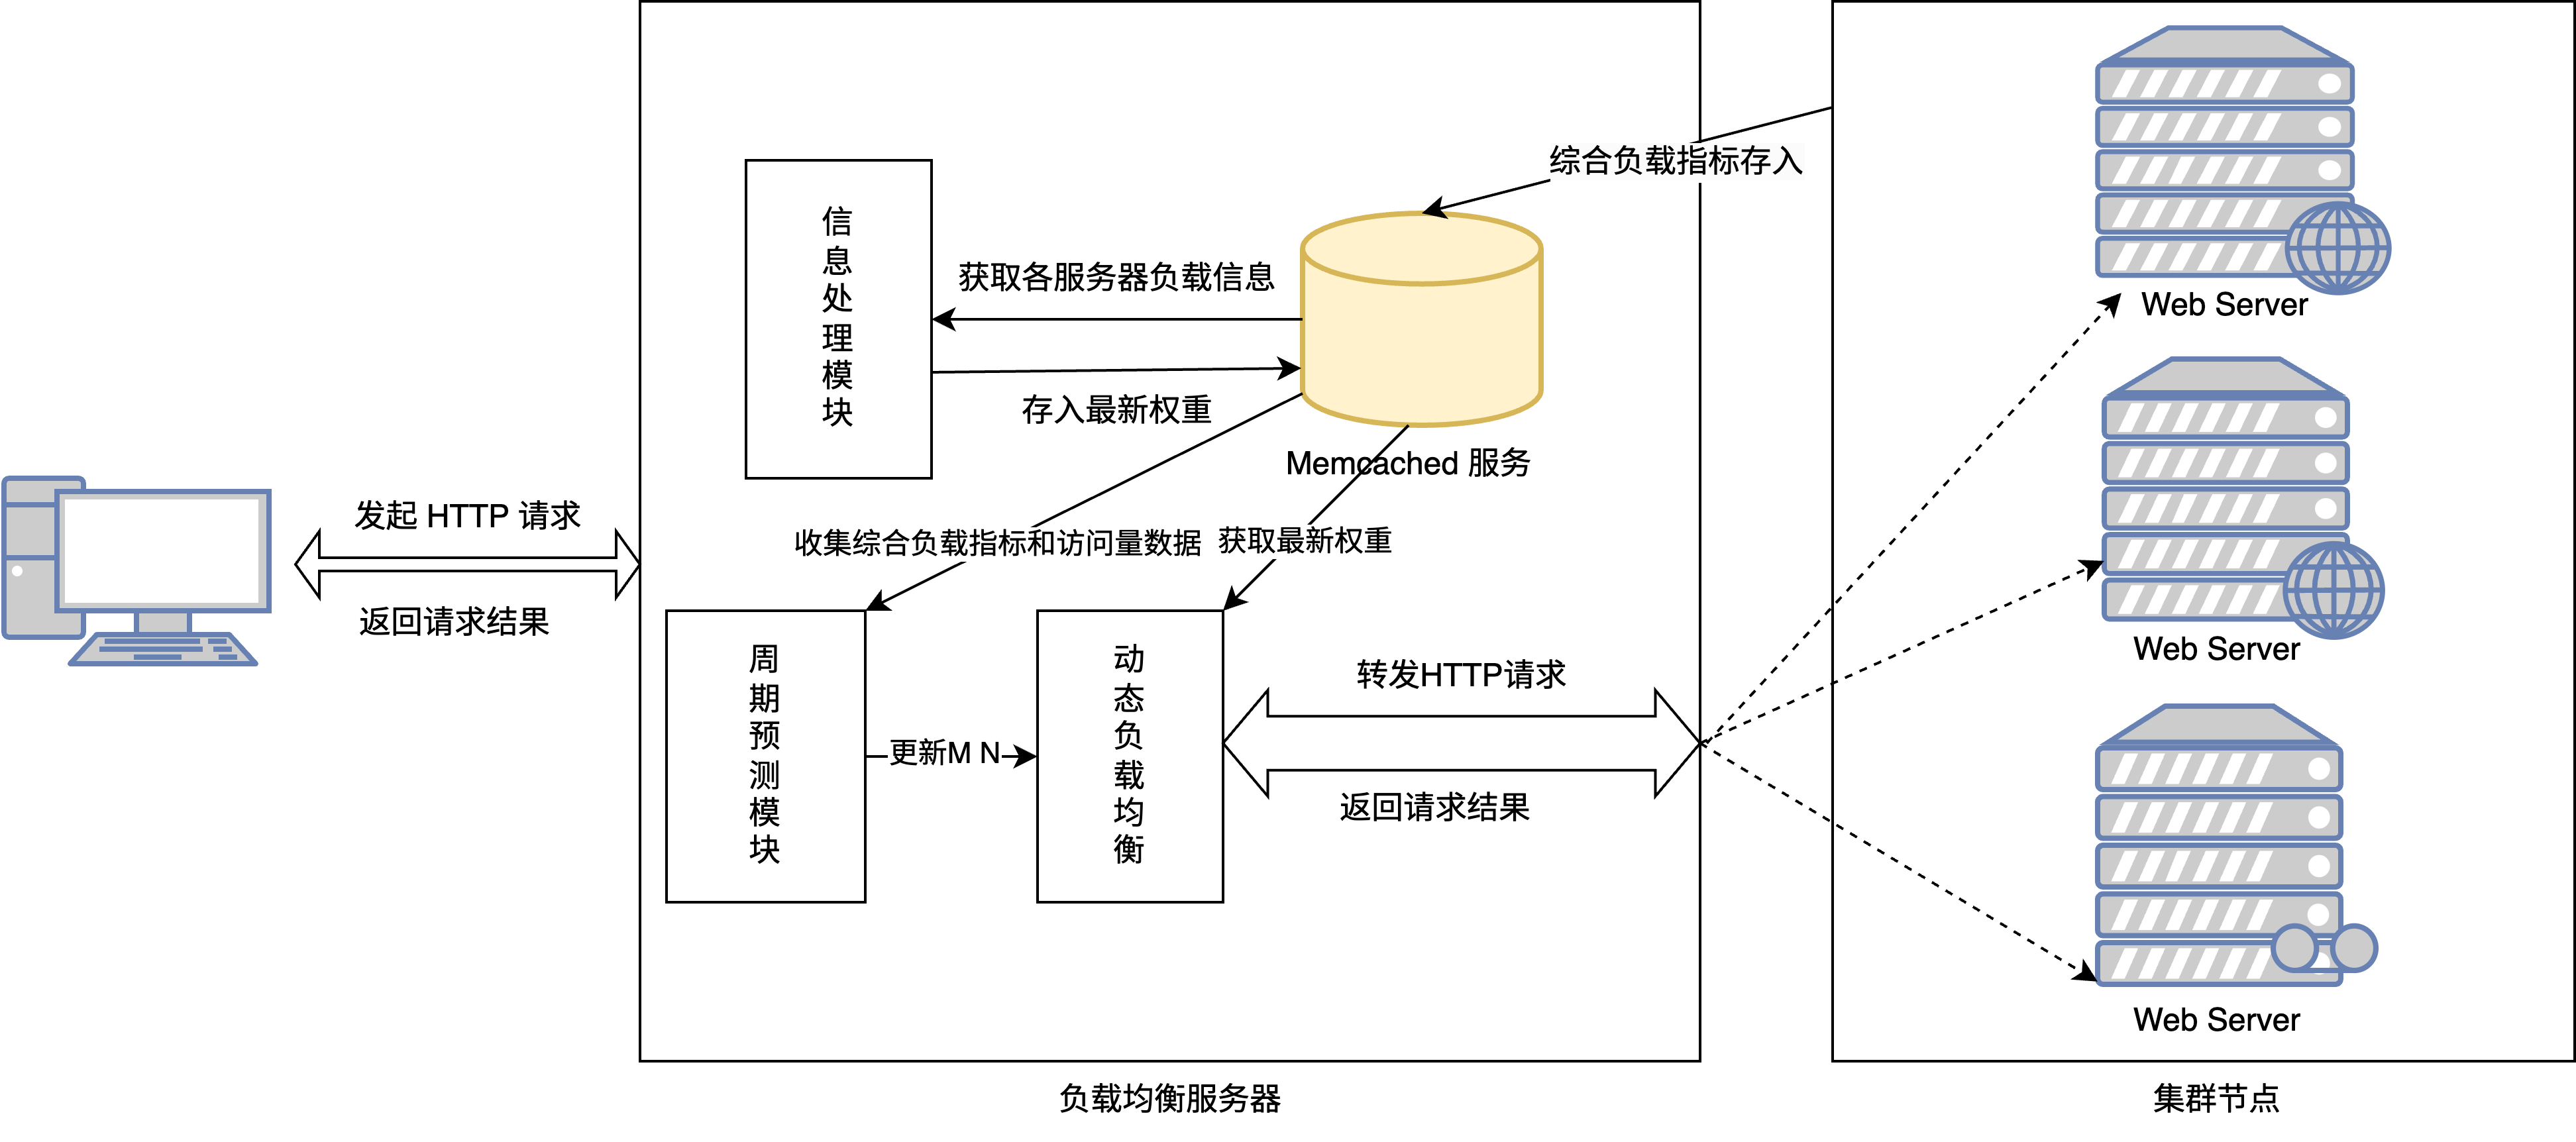
\includegraphics[width=\textwidth]{figures/landbalance_module.png}
  \caption{总体结构图}
  \label{total_structure_flow}
\end{figure}

当 client 用户发起 HTTP 请求任务到 Nginx 服务器,由 Nginx 服务器根据当前使用的负载均衡策略选取集群中某一个节点,把 client 发来的 HTTP 请求任务转发给该节点,该节点收到任务后进行处理,把数据发给 Nginx 服务器,Nginx 将收到的数据发回给客户端,客户端收到响应数据包,对数据进行处理并显示在网页上。改进后的平滑动态加权轮询算法流程如下图\ref{new_smoth_weight_balance}所示。

\begin{figure}[htbp]
  \centering
  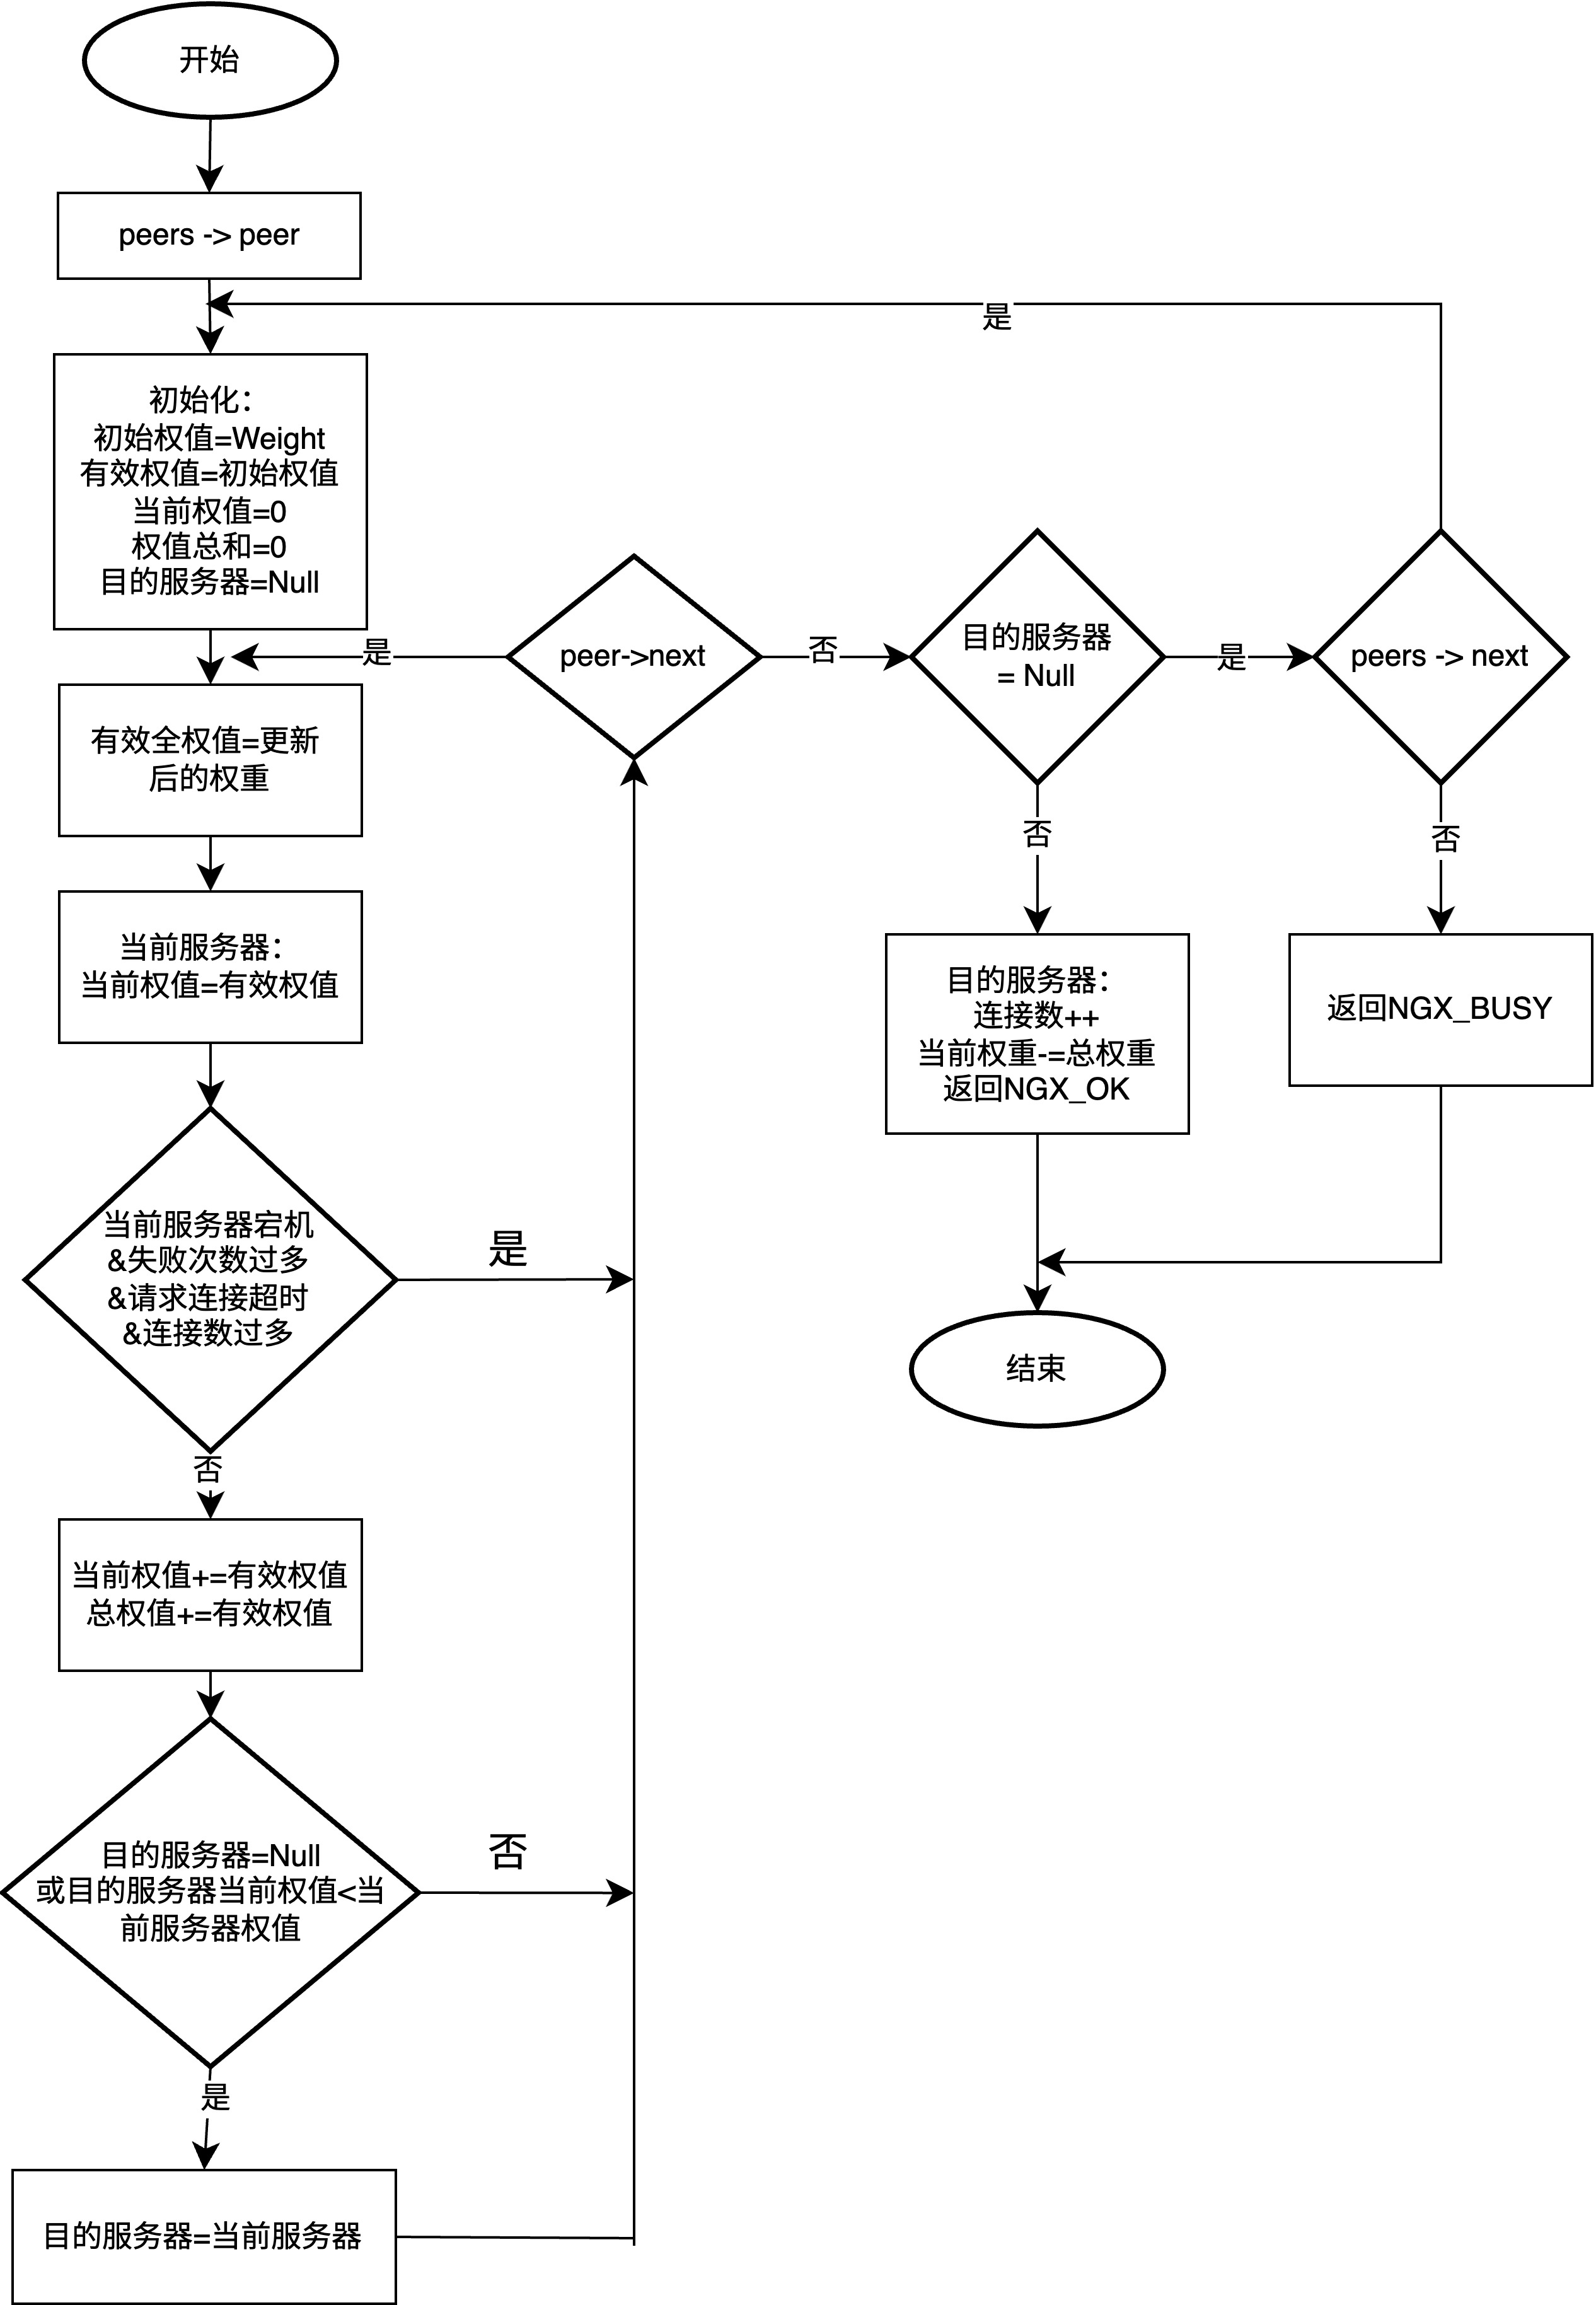
\includegraphics[width=\textwidth]{figures/new_smoth_weight_balance.jpg}
  \caption{改进后的平滑加权轮询算法流程图}
  \label{new_smoth_weight_balance}
\end{figure}

改进后的算法分为两个阶段:没有预测指标阶段和已有预测负载指标阶段。最开始没有合适的数据通过周期性预测处理模块对当前服务的相关访问量和服务器负载情况进行分析,则可以通过常规的平滑加权轮询算法完成初期任务。在第一个阶段中通过服务器负载信息收集模块对后端每一个节点此时的 CPU、IO、内存、网络带宽的利用率进行采集。
再将每个节点相关的负载数据交给服务器信息处理模块和周期性预测模块做相关数学分析,并通过公式(4.4)计算出各个节点出各个节点的总体负载情况,根据确定的阈值确定该节点是不是均衡,如果不均衡则更新该节点的权重数据。
等却动的阈值确定该节点是不是均衡,如果不均衡则更新某一节点的权重。当权重数据分析完毕后,由 Nginx 平滑加权轮询模块获取到最新的节点权重信息。
最后进行服务器配置以及权重初始化,该项初始化完成后,由 nginx\_http\_upstream\_get\_dynlb\_select\_peer 函数选择一台所有上游可用服务器中 current\_weight 最大的服务器对请求进行处理,如果所有节点都不符合条件,则选择 Nginx 自带的轮询算法。
当请求都处理完毕后调用 ngx\_http\_upstream\_free\_dynlb\_select\_peer 释放系统所占用的资源,提高算法的效率。第二个阶段则与第一个阶段类似,不过阈值和初始权重的调整会有所不同。

\section{负载均衡算法的优化}
通过第三章、第四章预测访问量的算法和剩余性能深度学习卷积神经网络的研究,有效的证明了算法的有效性和深度学习网络的优秀性能。通过对访问量的预测能够有效的在根据不同时间内分配合适的任务量,优化集群内的节点效率,有效降低集群的资金输入。通过时间卷积网络则可以很好的提取到不同时间段蕴藏的信息,同时得到了节点未来的负载情况,使得负载均衡器有效的分配合适的任务给合适的集群节点。
但是对于初期没有负载数据和访问量数据的问题,也需要值得重视,本节既是为了研究初期负载算法的优化。

第四章中通过主成分分析法分析了在已有数据情况下的公式(1.1)的权重参数,但是在没有数据之前仍然需要通过一定的分析得出一个较为合理的权重和综合负载情况的阈值。通过对不同论文的研究\cite{吴文辉2013编程计算层次分析法},本文选择了层次分析法来进行初期的权重参数的计算。

首先,需要构建出层次分析模型。将综合负载指标作为目标层,CPU、内存、网络带宽以及磁盘IO利用率指标作为准则层,层次分析模型结构如下图\ref{Layered_Analysis}所示。

\begin{figure}[htbp]
  \centering
  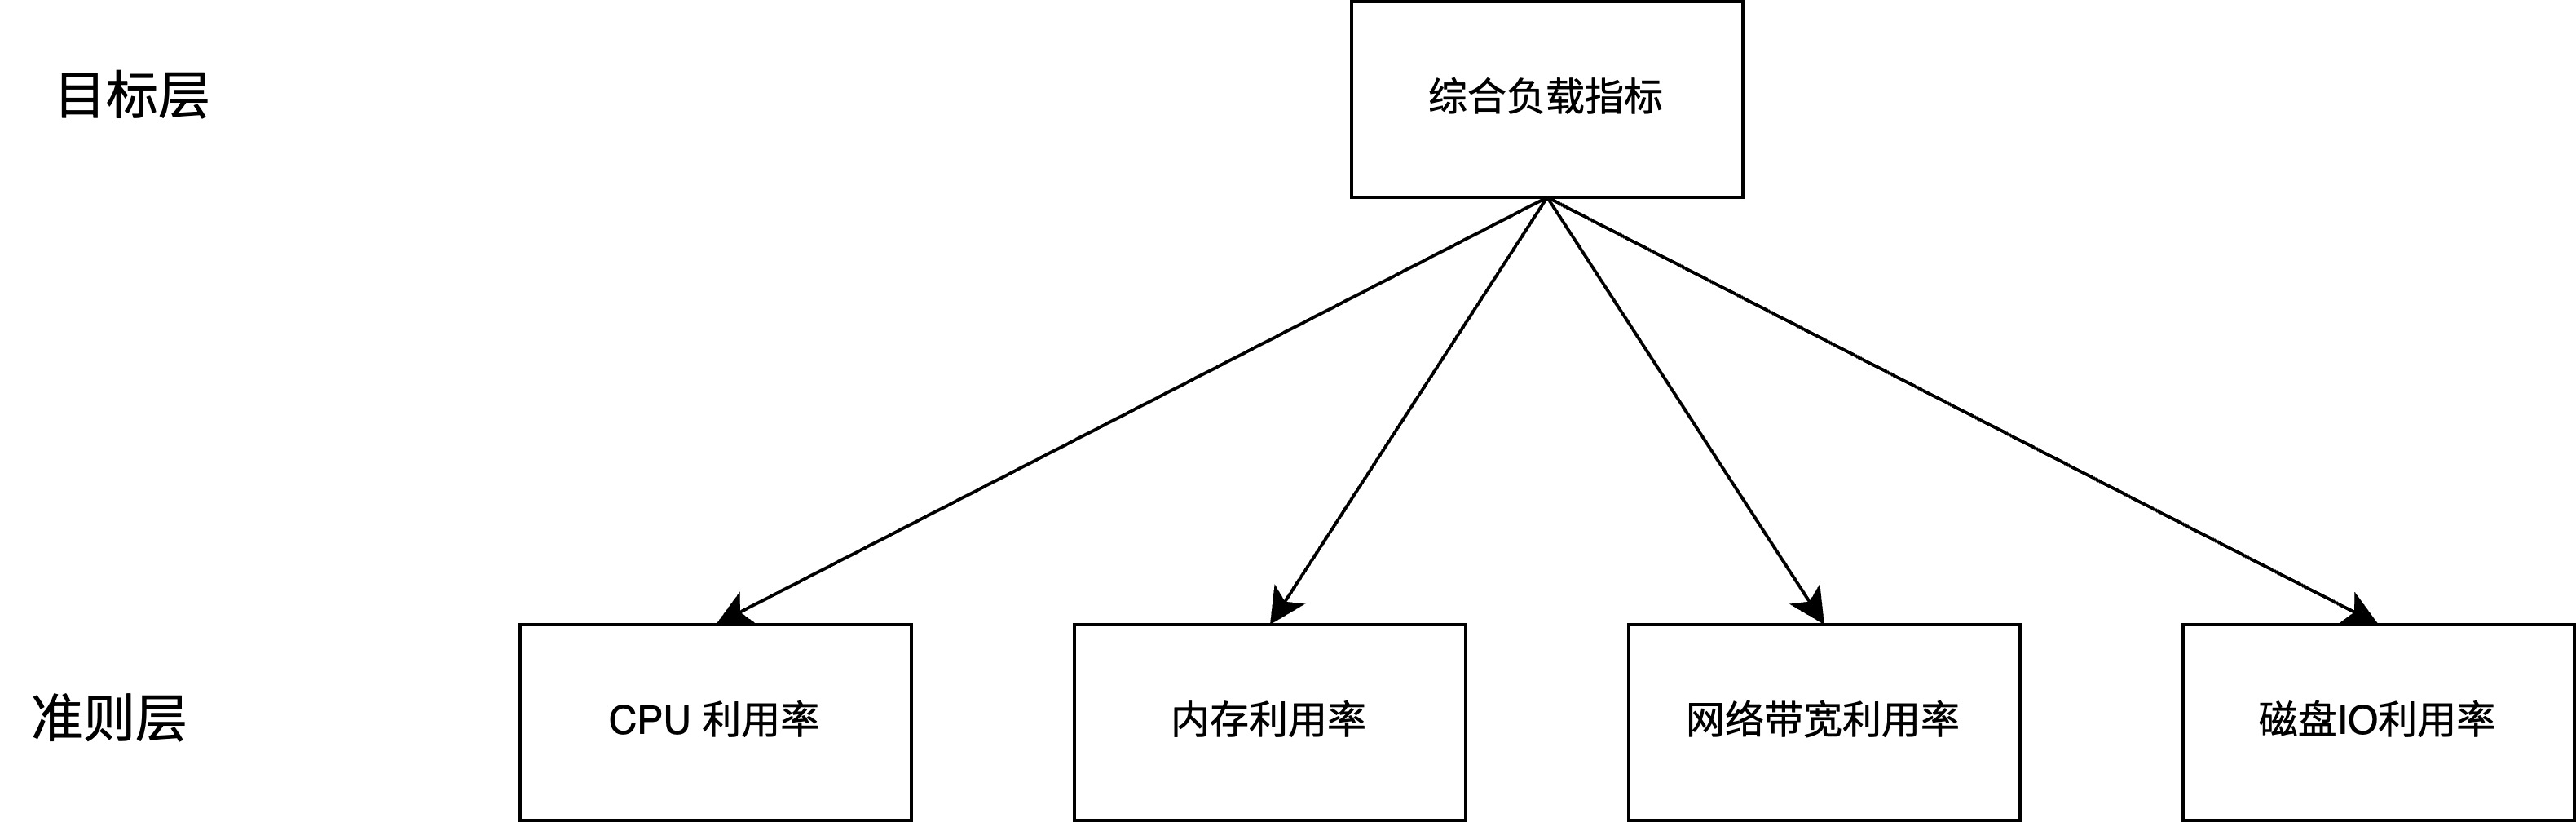
\includegraphics[width=\textwidth]{figures/Layered_Analysis.jpg}
  \caption{综合负载层次分析模型}
  \label{Layered_Analysis}
\end{figure}

采用 “1-9” 标度法,结合服务器测试情况构建判断矩阵。根据论文得知,CPU、内存利用率较高,而网络带宽与磁盘IO利用率相对较低\cite{吴陈2020基于Nginx的服务器集群负载均衡策略的研究与改进}。服务器对资源消耗标度表如下。

% \usepackage{tabularray}
\begin{longtblr}[
  caption = {服务器对资源消耗情况},
]{
  width = \linewidth,
  colspec = {Q[146]Q[331]Q[331]Q[113]Q[79]},
  vline{2-5} = {-}{},
  hline{1,6} = {-}{0.08em},
  hline{2} = {-}{},
}
Q   & CPU                                & Mem                                & Net & IO \\
CPU & 1                                  & 1                                  & 3   & 3  \\
Mem & 1                                  & 1                                  & 3   & 3  \\
Net & $\frac{1}{3}$ & $\frac{1}{3}$ & 1   & 1  \\
IO  & $\frac{1}{3}$ & $\frac{1}{3}$ & 1   & 1  
\end{longtblr}

于是,得到了判断矩阵:
\begin{equation}
  Q = \begin{bmatrix}
  1&  1&  3& 3\\
  1&  1&  3& 3\\
  1/3&  1/3&  1& 1\\
  1/3&  1/3&  1&1
\end{bmatrix}
\end{equation}

按照层次分析法的要求,得到了判断矩阵,通过合积法计算其近似特征向量。首先将矩阵(5.2)按照公式(5.3),再按列相加再做归一化,归一化的元素按行相加得到的结果处理后如下表所示。
\begin{equation}
  q_{ij}= \frac{q_{ij}}{\sum_{i=1}^{n}q_{ij} }(i,j = 1,2,\dots ,n)
\end{equation}

% \usepackage{tabularray}
\begin{longtblr}[
  caption = {对比表},
]{
  width = \linewidth,
  colspec = {Q[167]Q[179]Q[179]Q[179]Q[179]Q[113]},
  vlines,
  hline{1,6} = {-}{0.08em},
  hline{2} = {-}{},
}
Q   & CPU   & Mem   & Net   & IO    & ∑   \\
CPU & 0.375 & 0.375 & 0.375 & 0.375 & 1.5 \\
Mem & 0.375 & 0.375 & 0.375 & 0.375 & 1.5 \\
Net & 0.125 & 0.125 & 0.125 & 0.125 & 0.5 \\
IO  & 0.125 & 0.125 & 0.125 & 0.125 & 0.5 
\end{longtblr}

对上表自左向右最后一列元素进行归一化处理之后,即可得到特征向量 $M'=(M_1, M_2, M_3,\dots,M_n)^\mathbf{T}$的近似特征向量 $M'$。
\[
  M' = (0.375, 0.375, 0.125, 0.125)
\]
于是初始阶段的权重已经确定,则初期阶段综合负载决策函数为:
\begin{equation}
  X = 0.375\times(CPU) + 0.375 \times (Mem) + 0.125 \times (Net) + 0.125\times(IO)
\end{equation}

当节点的资源使用率达到了系统的瓶颈时,节点处理任务请求的效率就会明显下降,那么负载均衡器分配给节点的权重值就会减少。
通过表(2.2)可知,当节点的资源利用率评价为坏的时候,则可以认为此时节点负载过高。在初期阶段,此时总体剩余利用率可以通过公式(5.4)计算得到,在使用了周期性预测模块阶段则通过(4.4)计算得到,将该值设为 M,M 是判断节点负载是否平衡的条件,当 $T \ge M$  时,判断节点为高负载状态,则可以取阈值$N = L = 1 - H / 2$。

由于信息采集周期 $\mathbf{T}$ 对与负载信息收集模块和周期性预测模块有着很大的影响,对于负载信息采集模块来说,周期太短,可能导致信息收集太过于频繁而耗费过多的系统资源,周期太长,则会导致负载均衡服务器节点权重参数更新不及时,权重滞后。周期不能简单的通过定性进行分析得到,需要进行一定的实验对比,本文推荐使用 siege 来进行测试。

Siege是一款开源的压力测试工具,设计用于评估WEB应用在压力下的承受能力。可以根据配置对一个WEB站点进行多用户的并发访问,记录每个用户所有请求过程的相应时间,并在一定数量的并发访问下重复进行。对于不同业务的要求,可以选择不同的并发量,选择记录在指定文本文件内的链接访问不同类型的任务来模拟真实的负载情况。下面是推荐的并发量和任务类型。

% \usepackage{tabularray}
\begin{longtblr}[
  caption = {企业与任务类型},
]{
  width = \linewidth,
  colspec = {Q[323]Q[408]Q[146]},
  vline{3} = {-}{},
  hline{1,6} = {-}{0.08em},
  hline{2} = {-}{},
}
企业类型  & 并发量          & 任务 \\
小型企业  & 500-1000     & 文本 \\
中型企业  & 1000-5000    & 图片 \\
大型企业  & 10000-100000 & 音频 \\
超大型企业 & 100000-      & 视频 
\end{longtblr}
siege 的测试命令如下。
\noindent \begin{lstlisting}[caption={siege 的测试命令}]
siege -c 并发量 -r 重复次数 -f url.txt
\end{lstlisting}

其中url.txt 则是指定的任务类型,具体类型如下。
\noindent \begin{lstlisting}[caption={url.txt 请求任务类型}]
http://192.168.66.166/xx.jpg
http://192.168.66.166/xx.html
http://192.168.66.166/06.mpv
http://192.168.66.166/06.mp4
\end{lstlisting}

通过siege的测试可以得到不同周期 $T$ 下Nginx 的负载程度,通过对Nginx负载程度的定量分析,可以得到当前业务下最适合的周期 $T$。同时在周期预测阶段则可以选择每小时,每天,每月,每年作为整个周期进行拟合和预测。

在改进的动态负载均衡策略中,有两个重要部分,其一是使用合适的周期来收集各个服务器节点的剩余性能,并保存在 Memcached 服务中。Memcached 是一个分布式的告诉缓存系统,对于频繁获取负载信息的操作很有利,保证了收集数据的实时性,控制了资源的消耗。
其二,如果负载均衡器判断了集群某些节点负载不均衡后,如何调整各个节点的权重。

在本算法中,使用阻塞控制的思想来对权重进行调整。
拥塞控制是作用于网络的,它是防止过多的数据注入到网络中,避免出现网络负载过大的情况;常用的方法就是:( 1 )慢开始、拥塞避免( 2 )快重传、快恢复。本改进算法使用了,快重传,和快恢复算法。
常见的改进的动态负载均衡方法使用的是TCP Tahoe 算法,但是现在已经遭到抛弃。所以本算法使用的是 TCP Reno 算法。

快重传要求接收方在收到一个失序的报文段后就立即发出重复确认,而不要等到自己发送数据时捎带确认。快重传算法规定,发送方只要一连收到三个重复确认就应当立即重传对方尚未收到的报文段,而不必继续等待设置的重传计时器时间到期。
与快重传算法配套的还有快恢复算法,当发送方连续收到三个重复确认时,就执行“乘法减小”算法,把ssthresh门限减半(为了预防网络发生拥塞)。但是接下去并不执行慢开始算法,
考虑到如果网络出现拥塞的话就不会收到好几个重复的确认,所以发送方现在认为网络可能没有出现拥塞。所以此时不执行慢开始算法,而是将cwnd设置为ssthresh减半后的值,然后执行拥塞避免算法,使cwnd缓慢增大。下图是具体的拥塞控制窗口和传输轮次的关系表。下图\ref{tcp_reno}是改进的算法中,TCP Reno 的变化。

\begin{figure}[htbp]
  \centering
  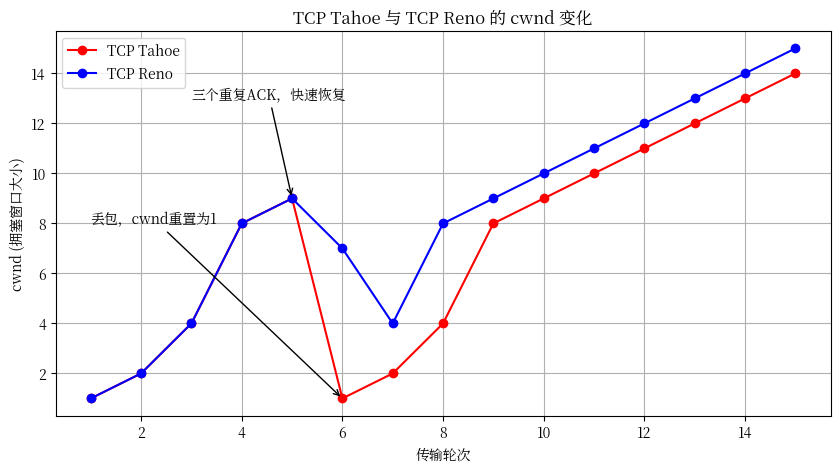
\includegraphics[width=\textwidth]{figures/tcp_reno.png}
  \caption{TCP Reno 的 cwnd 变化}
  \label{tcp_reno}
\end{figure}

TCP Reno 在 Tahoe 的基础上增加了快速恢复机制即快重传机制。在 Reno 中,当收到三个重复的 ACK 时(表示一个单一的数据包丢失),它不会像 Tahoe 那样直接进入慢启动阶段,而是进入快速恢复阶段。在这个阶段,它将阈值设为当前 cwnd 的一半,并将 cwnd 设置为新阈值加3个段的大小,然后进行拥塞避免算法。如果又出现超时,则会和 Tahoe 一样,将 cwnd 设为1,重新开始慢启动过程。Reno 的这种机制可以在某些丢包情况下避免 cwnd 的大幅度减少,使得网络能够更快地恢复到有效的传输状态。从而使的负载均衡节点更有效的调整节点的权重

根据这种思想,本文想去了服务器节点的综合负载指标这一指标作为判断负载时的条件,并设置一个阈值 $N$ 作为改进的动态轮询算法的权重调整门限,值 $M$ 判断节点是否负载均衡的条件。但是,初期阶段根据服务器信息处理模块收集到的信息来进行判断具有滞后性。所以在预测阶段能使用深度学习算法来预测节点综合负载指标来作为判断标准,获取所有节点下一时间段的综合负载情况,若判断存在服务器节点下一时间会变成高负载状态,则将下一时刻判断为负载不均衡的节点进行权重调整,调整方式为$W_j = 1000 \times U_j / \sum U_i$,$\sum U_i$ 表示下一时刻所有负载不均衡节点综合负载指标的和,$U_j$为第 $j$ 个且被判断为下一时刻负载不均衡的节点。并将节点的权重信息存入 Memcached 服务,对于低负载节点权重,将其调整为 $W_{Cj} = W_j - 2^n$,$n$ 为权重调整次数,直至权重变为初始权重。

持续观察高负载节点节点负载状况,在该服务器节点的综合指标 $X < N$ 当前权重值小于初始权重时,使该节点的权重为 $W_{Cj} = W_j + 2^n$,$n$ 是调整次数,若此过程中当前权重增长值等于初始权重大小,则调制权重增长。单个服务器节点的综合负载指标 $X \ge N$ 且当前权重小于初始权重时,停止次节点的指数增长,使其呈现线性增长。$W_{Cj} = W_j + 2^k$,$k$ 为停止指数增长此刻权重调整的次数。若在此过程中权重带到初始权重值,则停止权重增长,或者该节点再次被判断为下一时刻处于高负载状态,则再将权重进行调整。在节点的权重信息调整过程中,持续更新其权重值,并录入至 Memcached 中。其高负载节点权重调整流程图如图\ref{contral_weight}所示。

\begin{figure}[htbp]
  \centering
  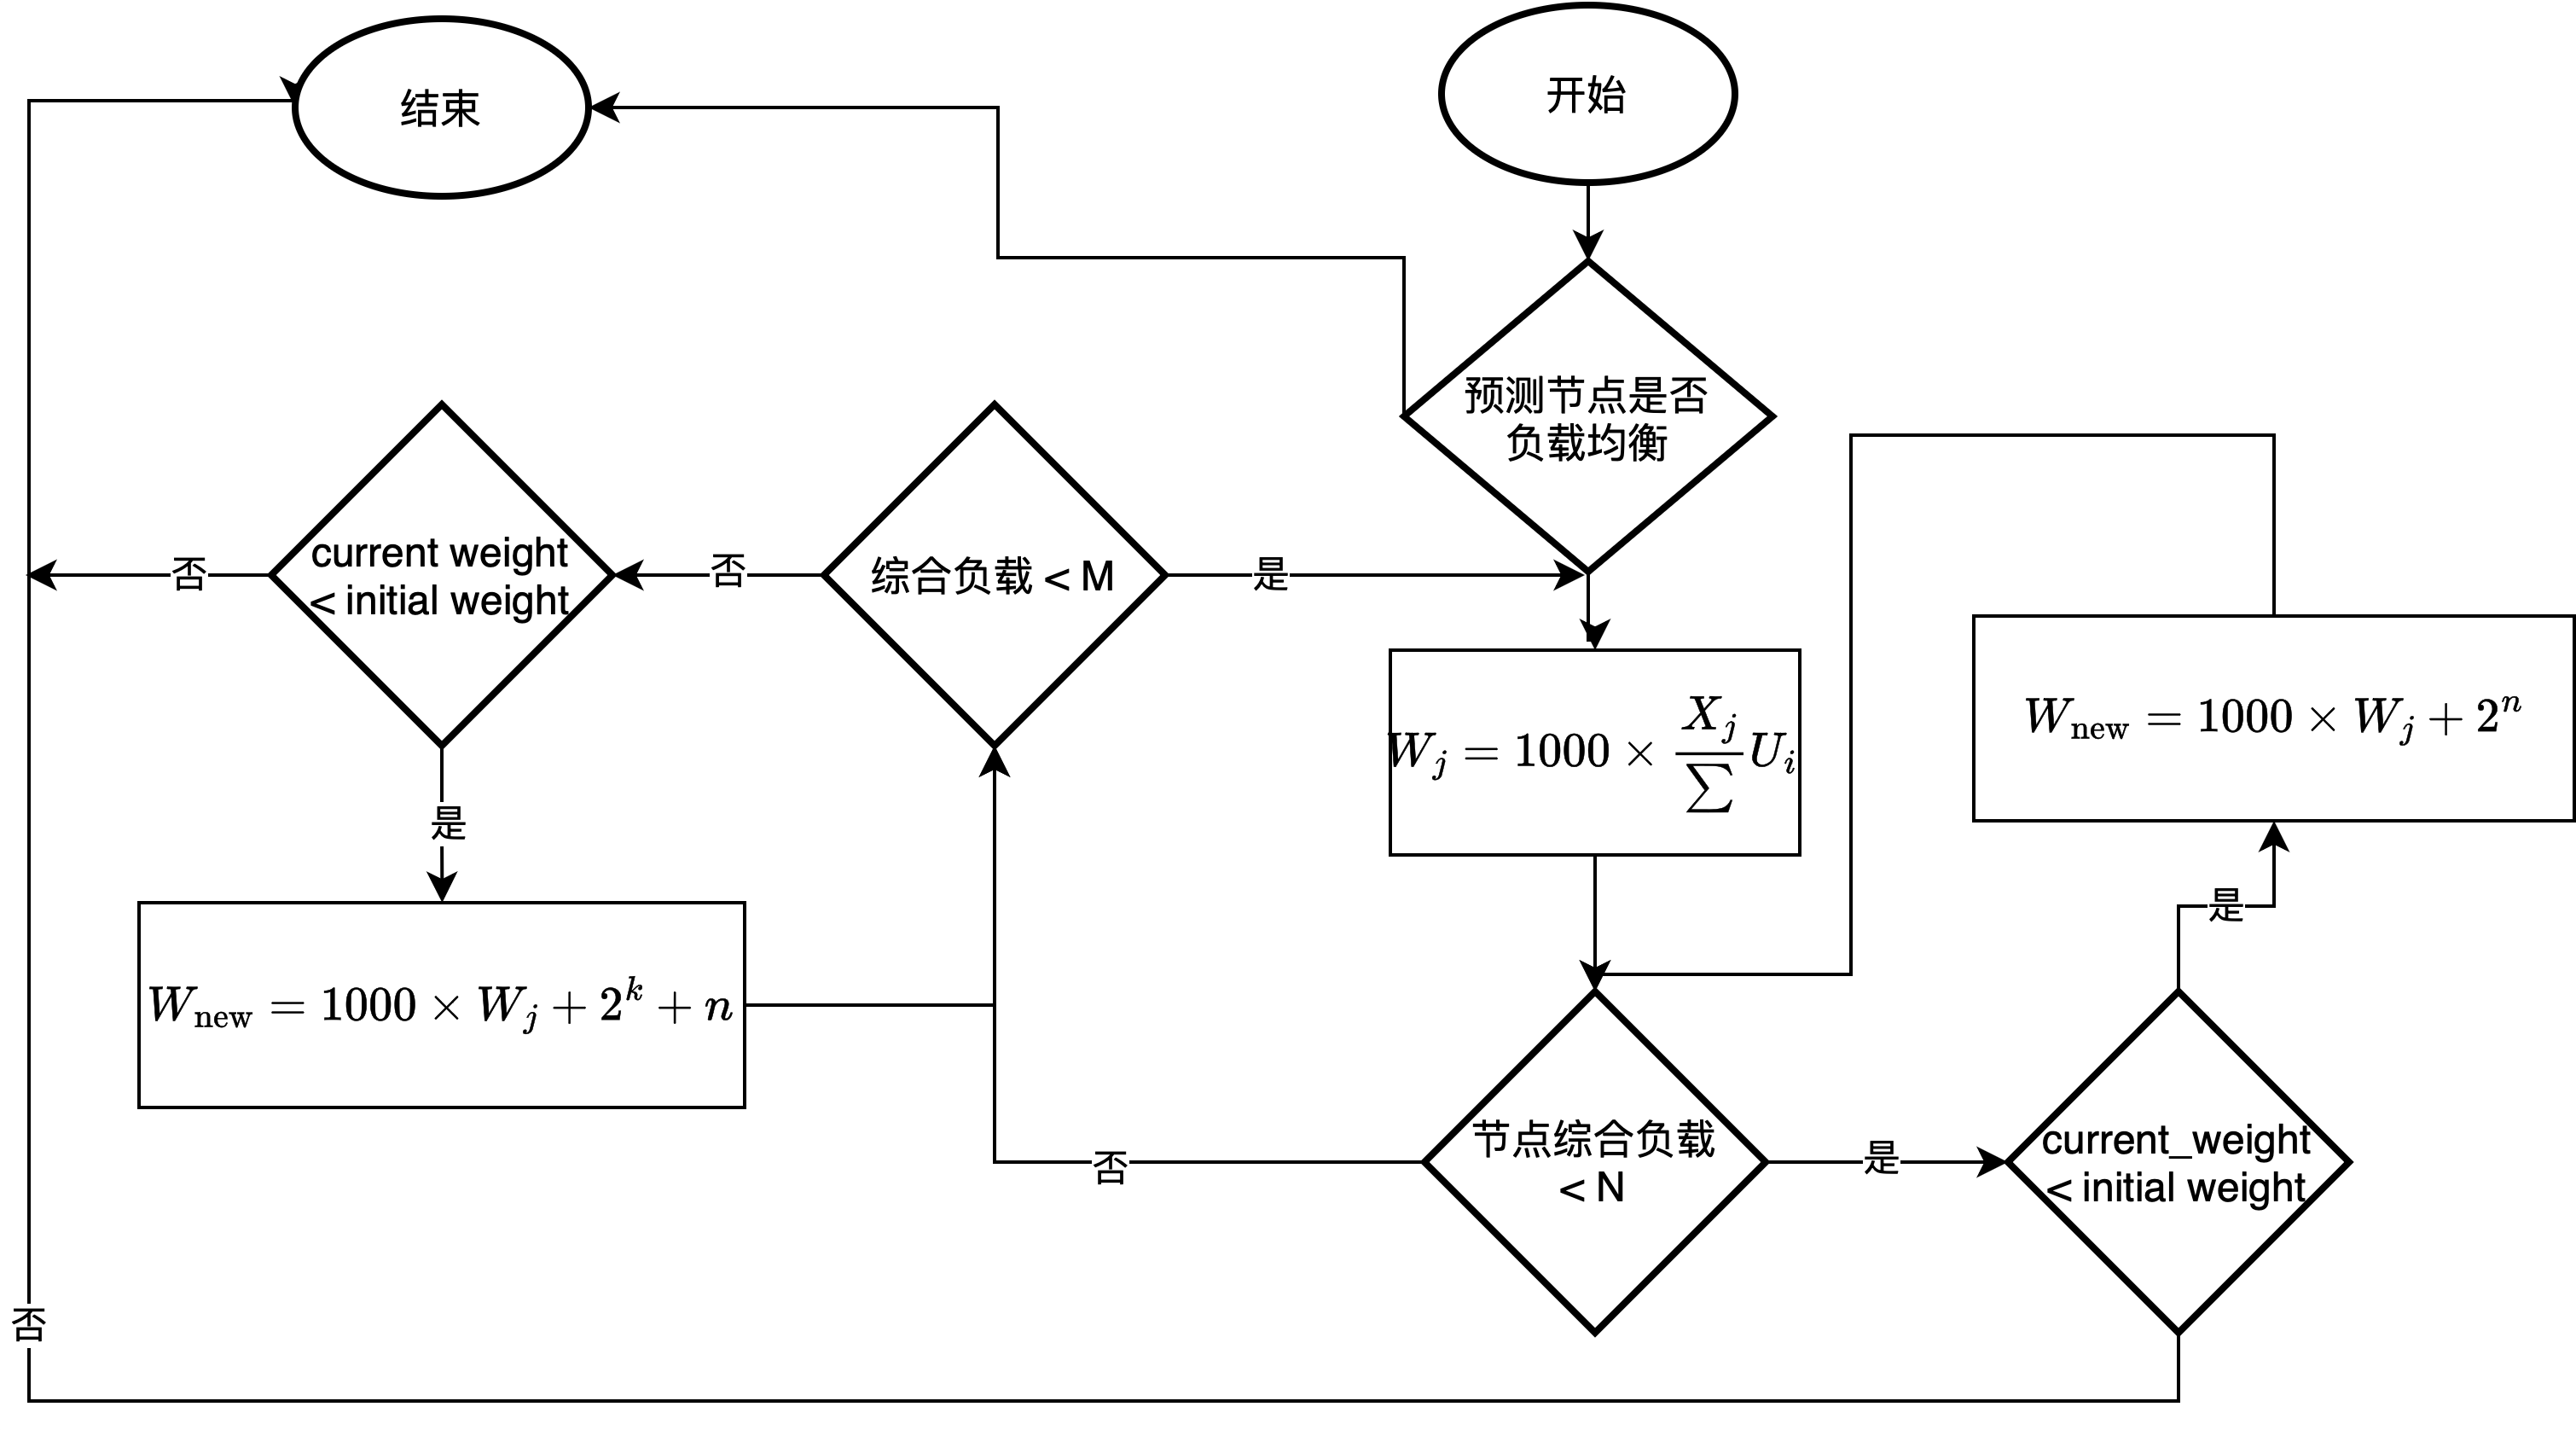
\includegraphics[width=.9\textwidth]{figures/change_weight.png}
  \caption{基于拥塞控制思想的权重调整流程}
  \label{contral_weight}
\end{figure}

\section{本章总结}
在本章中,通过研究常规的动态负载均衡方案的不足,提出了与预测模型相结合的动态负载均衡方案。其中包含两个阶段,初期阶段和预测阶段,很好的解决了改进算法在没有数据时的负载均衡方案,提出了收集周期 $T$ 和初期阶段的初始权重,和调整权重的阈值 $N$,同时使用 TCP Reno 方案优化了负载均衡器调整权重时的性能。
